%%%% Modified version of the Better poster example
%%%% by Tim Smith

%%%% Better Poster latex template example v1.0 (2019/04/04)
%%%% GNU General Public License v3.0
%%%% Rafael Bailo
%%%% https://github.com/rafaelbailo/betterposter-latex-template
%%%%
%%%% Original design from Mike Morrison
%%%% https://twitter.com/mikemorrison

\documentclass[a0paper]{betterposter}

\usepackage{../rnn}
\usepackage{tikz}
\usepackage{tcolorbox}
\usepackage{setspace}
\usepackage{ragged2e}
\usepackage{overpic}

% --- Tikz stuff
\usetikzlibrary{shapes.geometric, hobby, decorations.pathreplacing, calc}
\usetikzlibrary{arrows, arrows.meta}

\definecolor{sapphire}{HTML}{0F52BA}
\definecolor{emerald}{HTML}{27AE60} % 229954} % 50C878}

% bibentry has \nobibliography
%\usepackage{bibentry}

\usepackage[style=apa]{biblatex}
\addbibresource{../references.bib}
\renewcommand*{\finalnamedelim}{%
   \ifnumgreater{\value{liststop}}{2}{\finalandcomma}{}%
   \addspace\&\space}

% Remove default references section title
\renewcommand\refname{}

%%%% Uncomment the following commands to customise the format

%% Setting the width of columns
% Left column
\setlength{\leftbarwidth}{0.3\paperwidth}
% Right column
\setlength{\rightbarwidth}{0.3\paperwidth}

%% Setting the column margins
% Vertical margin
\setlength{\columnmarginvertical}{0.031\paperheight} % 1.03 inches with a0paper
% Horizontal margin
\setlength{\columnmarginhorizontal}{0.022\paperwidth} % 1.03 inches with a0paper
% Vertical margin for the main column
\setlength{\maincolumnmarginvertical}{0.07\paperheight} % this seems to be in addition to  standard margin
% Horizontal margin for the main column
\setlength{\maincolumnmarginhorizontal}{0.02\paperwidth}

%% Changing font sizes
% Text font
\renewcommand{\fontsizestandard}{\fontsize{36.00}{44.2} \selectfont}
\newcommand{\fontsizecite}{\fontsize{30.00}{42.0} \selectfont}
% Main column font
\renewcommand{\fontsizemain}{\fontsize{42.00}{50.50} \selectfont}
% Title font
\renewcommand{\fontsizetitle}{\fontsize{72.00}{108.00} \selectfont}
% Author font
\renewcommand{\fontsizeauthor}{\fontsize{48.00}{68.00} \selectfont}
% Section font
\renewcommand{\fontsizesection}{\fontsize{48.00}{68.00} \selectfont}
% Institution font
\newcommand{\fontsizeinstitution}{\fontsize{28.00}{38.00} \selectfont}
% Citation fonts
\let\realcite\parencite
\renewcommand*{\cite}[1]{{\fontsizecite\realcite{#1}}}
\newcommand{\citeps}[1]{{\fontsizeinstitution\realcite{#1}}}

%% Changing font sizes for a specific text segment
% Place the text inside brackets:
% {\fontsize{28}{35} \selectfont Your text goes here}

%% Changing colours
% Background of side columns
%\renewcommand{\columnbackgroundcolor}{black}
% Font of side columns
%\renewcommand{\columnfontcolor}{gray}
% Background of main column
\renewcommand{\maincolumnbackgroundcolor}{white}
%\renewcommand{\maincolumnbackgroundcolor}{theory}
%\renewcommand{\maincolumnbackgroundcolor}{methods}
%\renewcommand{\maincolumnbackgroundcolor}{intervention}
% Font of main column
\renewcommand{\maincolumnfontcolor}{black}

\begin{document}
\betterposter{
    \begin{FlushLeft}
        
\begin{tcolorbox}[width=\textwidth,
    colframe=sapphire,
    colback=white,
    arc=24pt,
    boxrule=5pt,
    boxsep=0.5em]


    \begin{minipage}{\textwidth}
        \centering
        \fontsizesection
        \textbf{Takeaway 1: Impact of Temporal Subsampling}
    \end{minipage}
    \vspace{1em}

    \begin{minipage}{\textwidth}
        \centering
        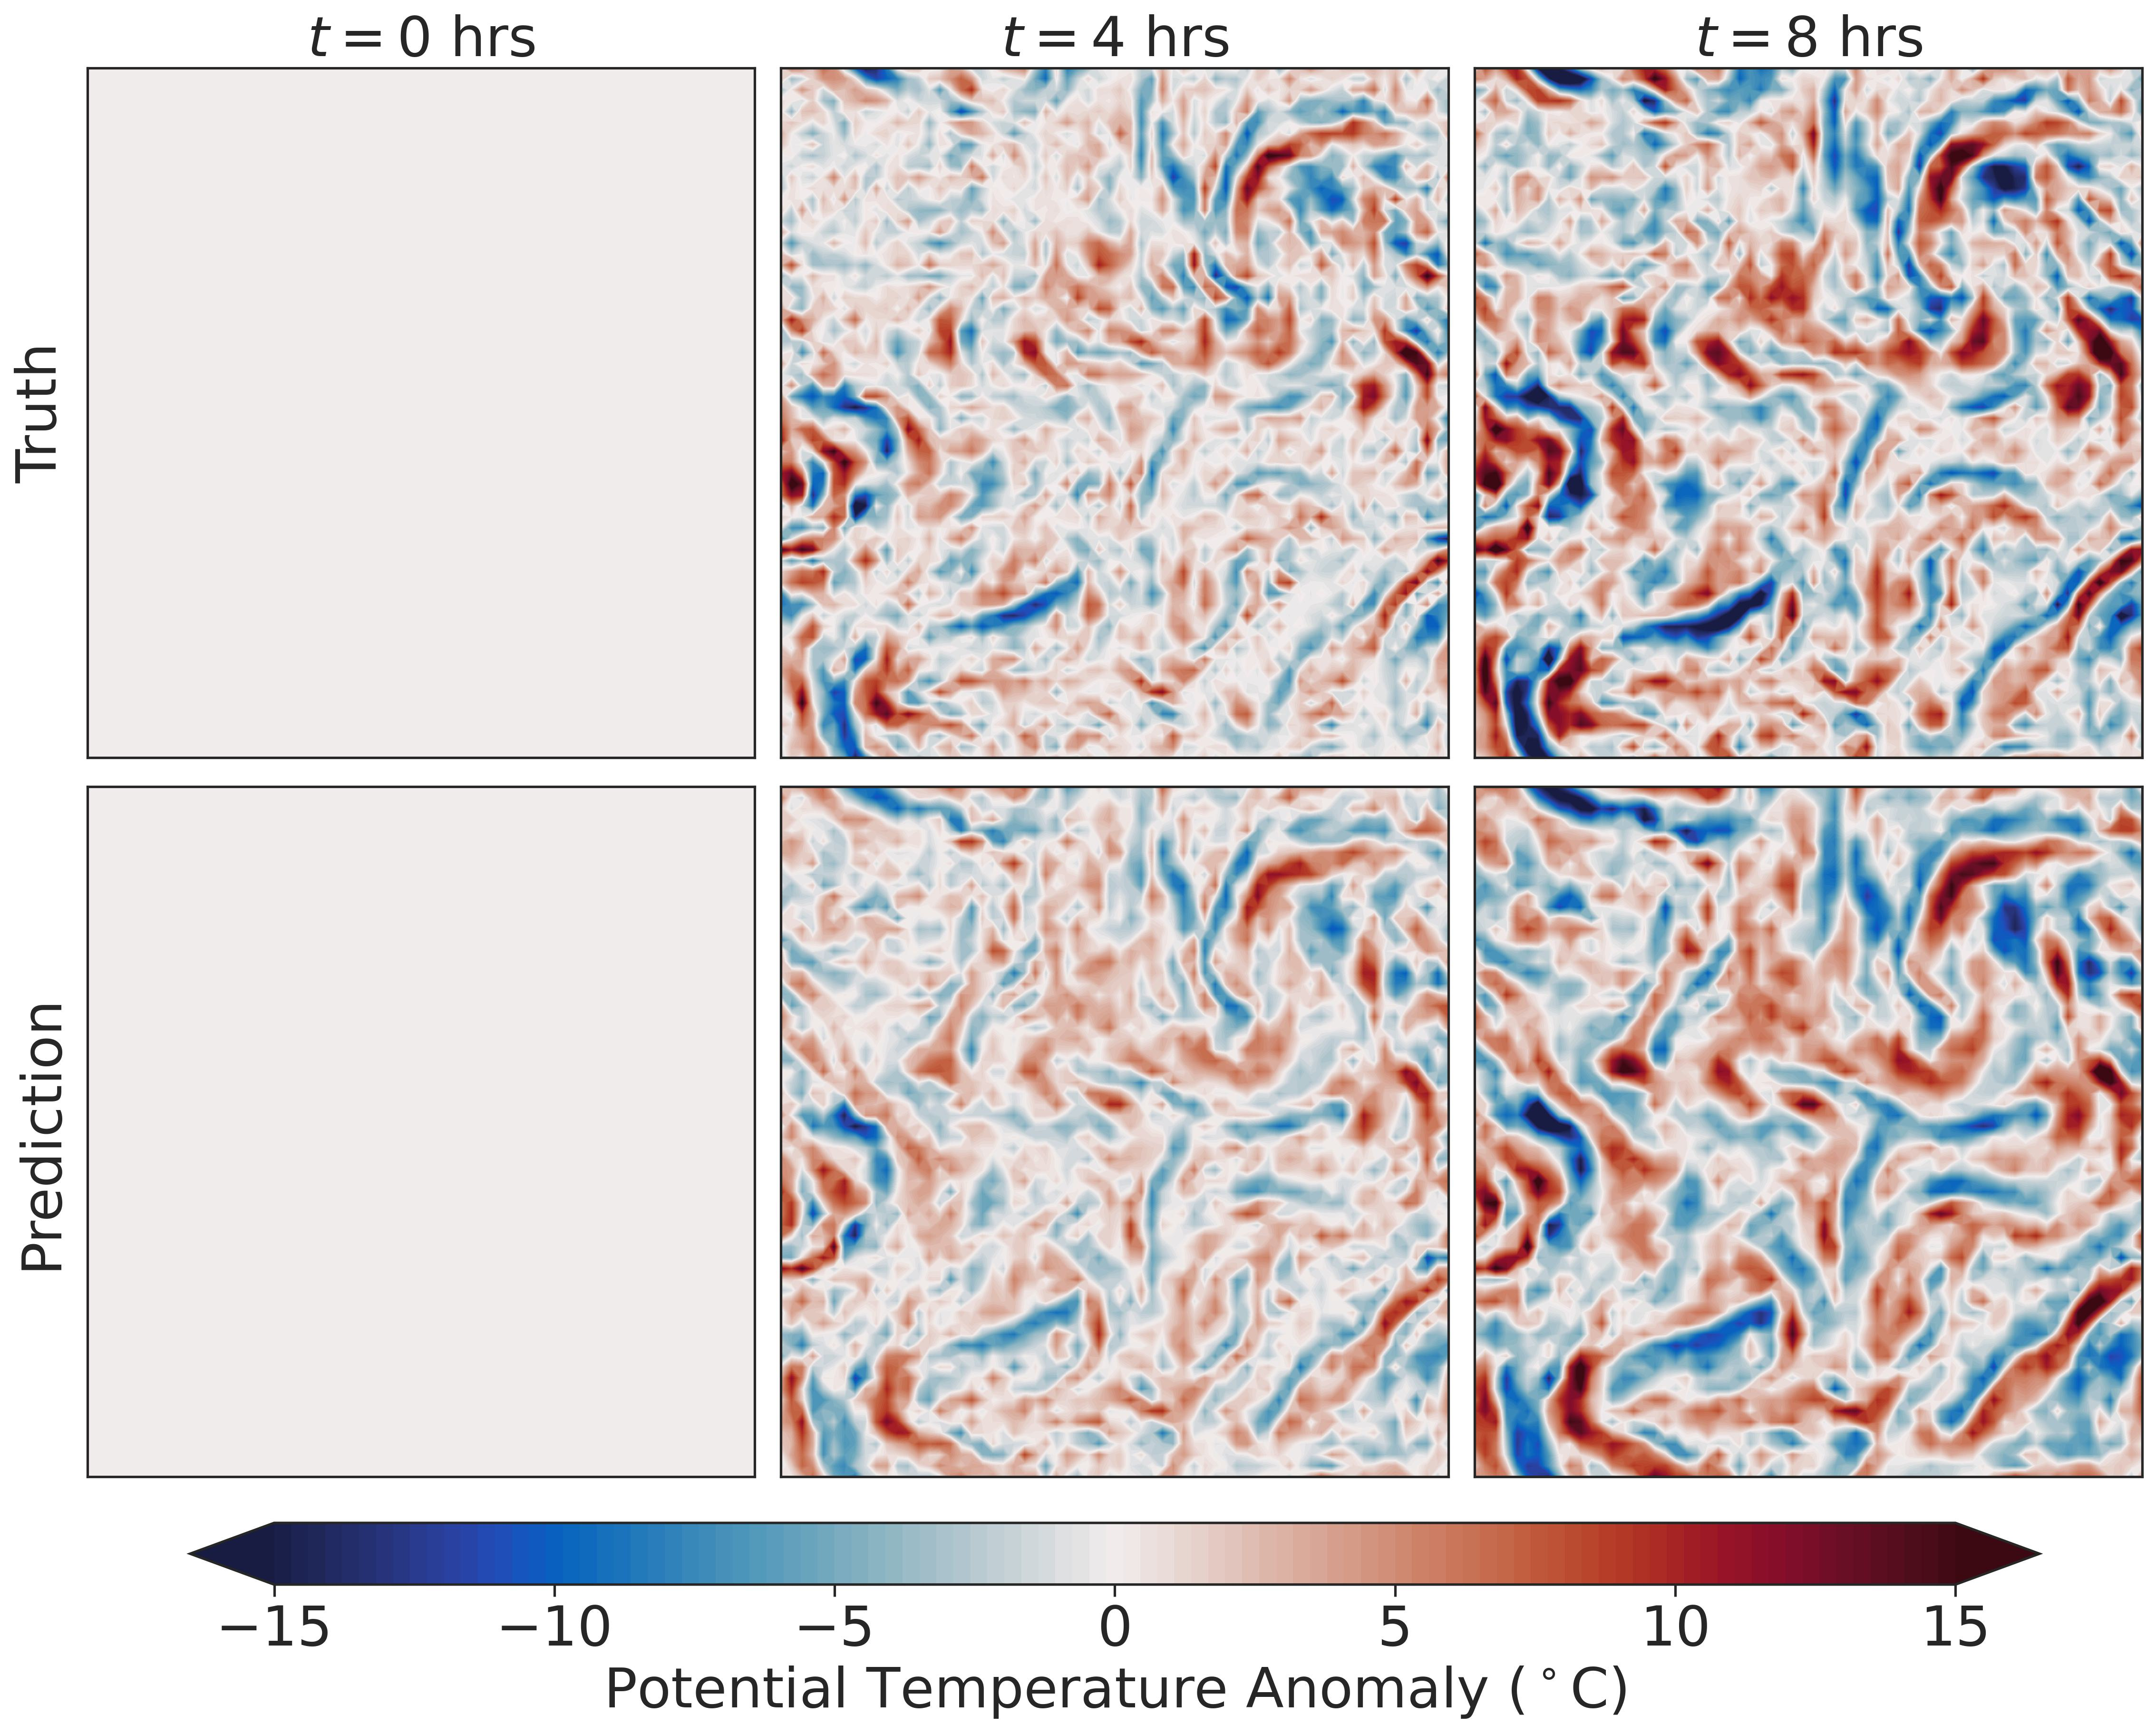
\includegraphics[width=.65\textwidth]{../../figures/nvar-diff-4800dt-nice.jpg}
        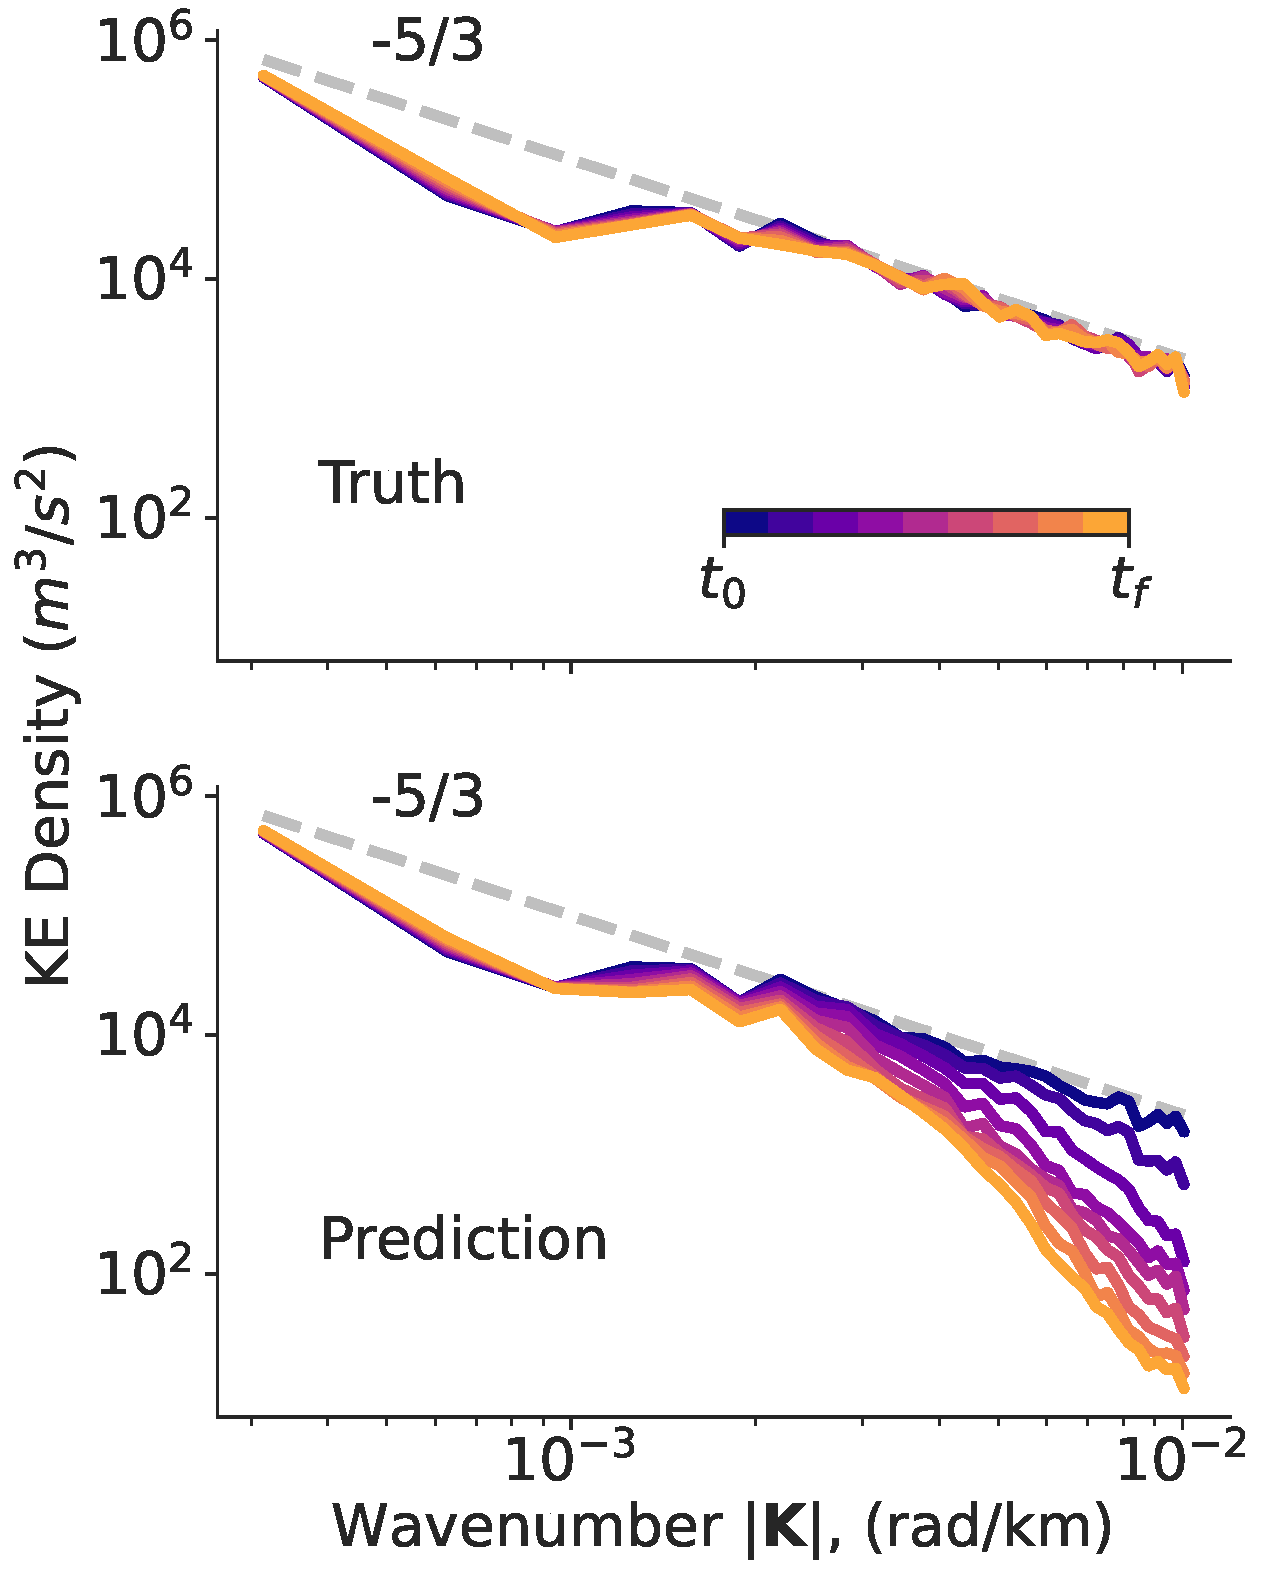
\includegraphics[width=.34\textwidth,trim={0, -2em, 0, 0}, clip]{
        ../../figures/spectrum_4800dt_nice.pdf}
    \end{minipage}

    \vspace{1.5em}
    \begin{minipage}{\textwidth}
        \begin{itemize}
            \item Prediction shows good qualitative resemblance of flow,
                despite simplistic NVAR setup
            \item Subsampling removes small scale features, resembling
                CFL-type barrier
            \item Many ML models use subsampled reanalysis output for
                training. This subsampling will contribute to a reduced
                ``effective'' resolution.
        \end{itemize}
    \end{minipage}
\end{tcolorbox}


\vfill
\begin{tcolorbox}[width=\textwidth,
    colframe=sapphire,
    colback=white,
    arc=24pt,
    boxrule=5pt,
    boxsep=0.5em]


   \begin{minipage}{\textwidth}
       \centering
       \fontsizesection
       \textbf{Takeaway 2: Impact of Memory in RNNs}
   \end{minipage}
   \vspace{1em}

    \begin{minipage}{\textwidth}
        \centering
        \includegraphics[width=.45\textwidth]{../../figures/nvar-rmse-vs-lag-1200dt.pdf}
        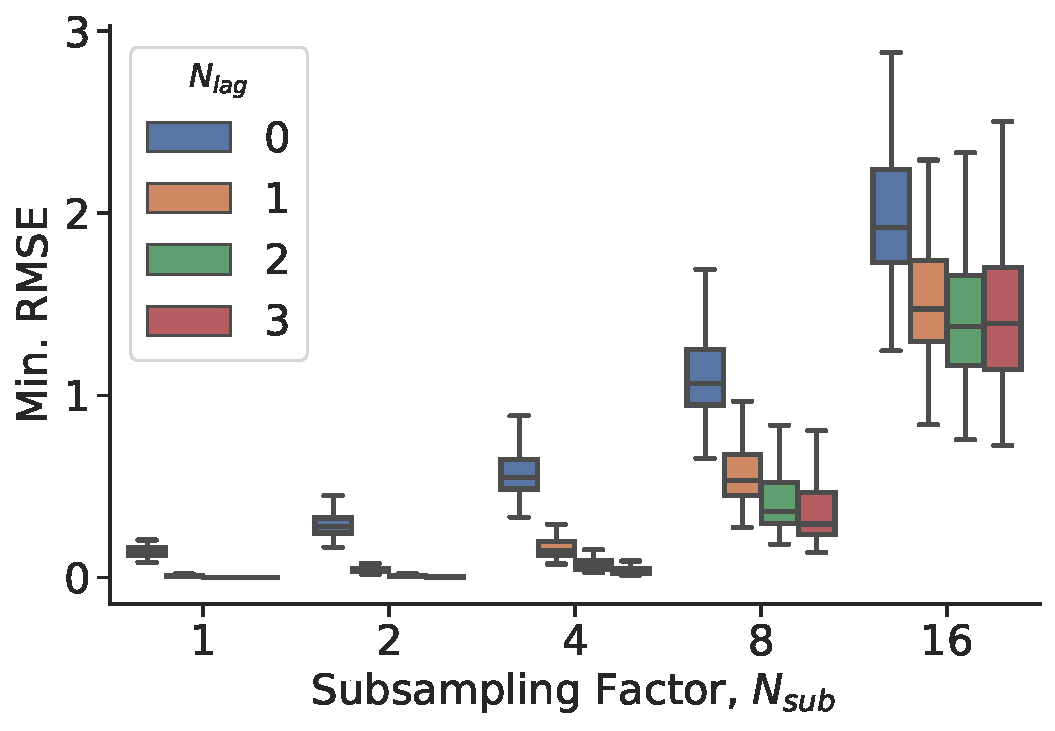
\includegraphics[width=.45\textwidth]{../../figures/nvar-mrmse-vs-lag-050samples.pdf}
    \end{minipage}

    \vspace{1.5em}
    \begin{minipage}{\textwidth}
        \begin{itemize}
            \item Adding time lagged states (i.e., increasing memory)
                improves prediction skill, albeit with diminishing returns
            \item For certain subsampling factors, prediction skill
                approaches that of RNN trained on model timestep
            \item Quadratic NVAR does not capture nonlinear
                interactions between time-lagged states
            \item Corroborates \cite{zhang_catch-22_2022}: small
                uncertainties/inaccuracies in NVAR nonlinearity are
                detrimental to prediction skill
        \end{itemize}
    \end{minipage}
\end{tcolorbox}

    \end{FlushLeft}
}{
    \begin{FlushLeft}
        \title{Recurrent Neural Network Emulation of Turbulent Geophysical Fluids}

\author{Timothy A. Smith$^{1,2}$, \texttt{tim.smith@noaa.gov}\vspace{-.25em}}

\begin{minipage}{.5\textwidth}
    \vspace{-1.25em}
    \author{Stephen G. Penny$^{3}$\vspace{.25em}}
    \author{Jason A. Platt$^{4}$\vspace{.25em}}
    \author{Tse-Chun Chen$^{1,2}$}
\end{minipage}
\begin{minipage}{.5\textwidth}
    \institution{\fontsizeinstitution
        \justifying
        $^1$CIRES, CU Boulder \\
        $^2$NOAA, Physical Sciences Lab (PSL) \\
        $^3$Sofar Ocean Technologies\\
        $^4$University of California, San Diego
    }
\end{minipage}

\section{Motivating Goals}
\begin{itemize}
    \item Develop cheap emulator to replace GCMs in Data Assimilation (DA)
    \item Enable increased ensemble size and/or resolution
\end{itemize}

\section{Why use RNNs?}
\begin{itemize}
    \item Recurrent Neural Networks (RNNs) discussed here have achieved excellent
        prediction skill emulating chaotic dynamics \cite{platt_systematic_2022}
    \item For low dimensional chaotic systems, successful
\end{itemize}

\hfill\begin{minipage}{.95\textwidth}
    \begin{enumerate}
        \item Lyapunov spectrum reproduction\cite{pathak_using_2017}
        \item Numerical model replacement in DA algorithms
            \cite{penny_integrating_2022}
    \end{enumerate}
\end{minipage}

\section{Questions to be Addressed}
\begin{itemize}
    \item What scales can we truly resolve with neural network emulators?
    \item How do fundamental data decisions impact performance?
    \item How much does RNN memory benefit performance?
\end{itemize}

\section{Surface Quasi-Geostrophic Turbulence}

\vspace{1em}
\begin{minipage}{.6\textwidth}
    \begin{tikzpicture}[scale=1]
        \node(upper) at (-1, 1){
            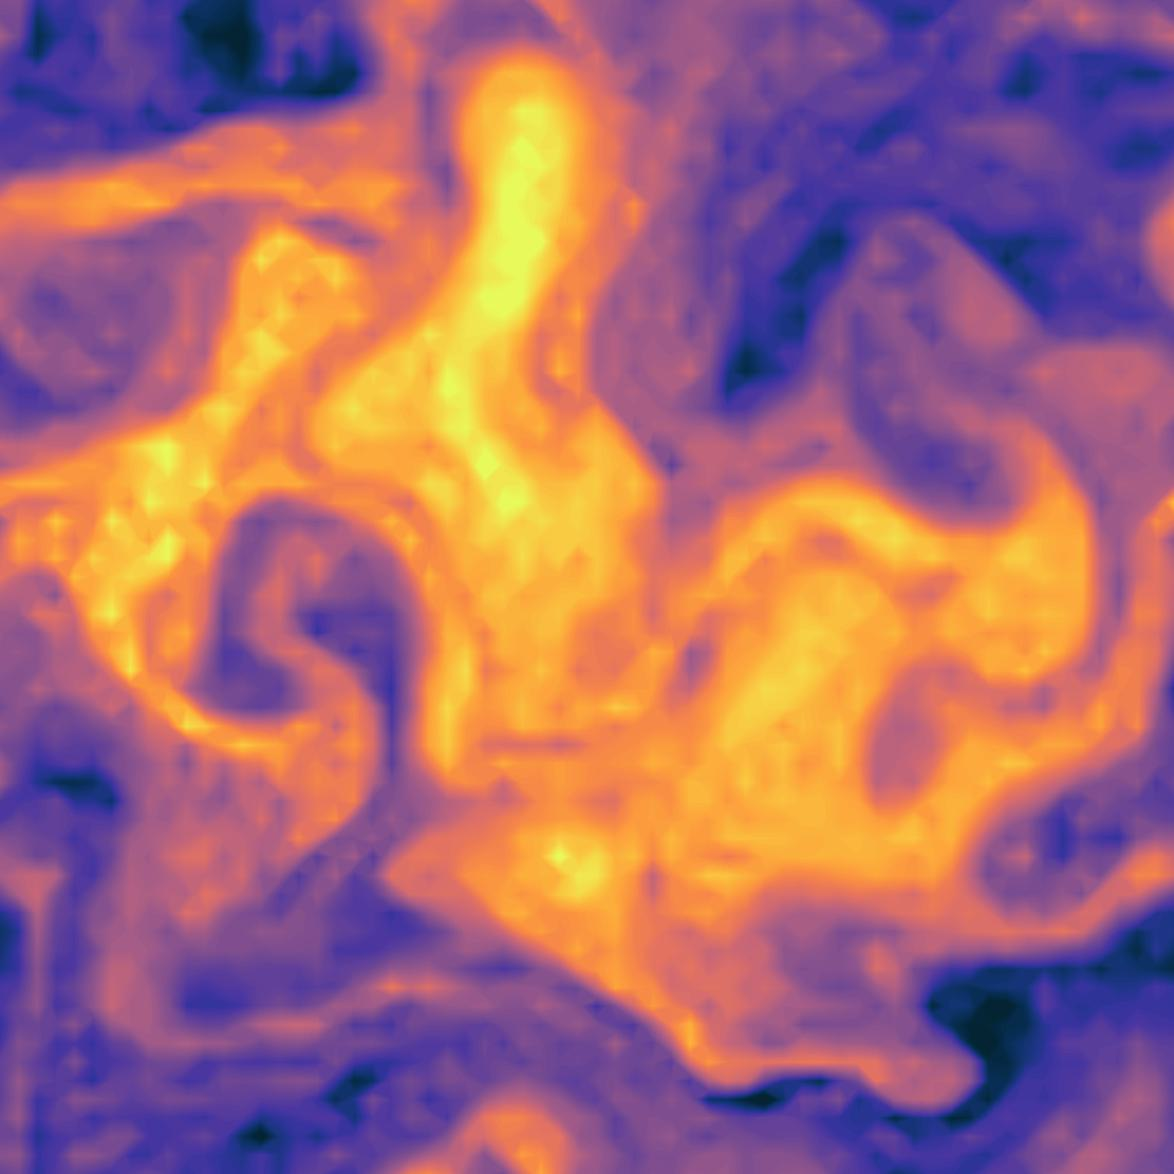
\includegraphics[width=.74\textwidth]{../../figures/theta-z1.jpg}
        };
        \node(lower) at (1, -1){
            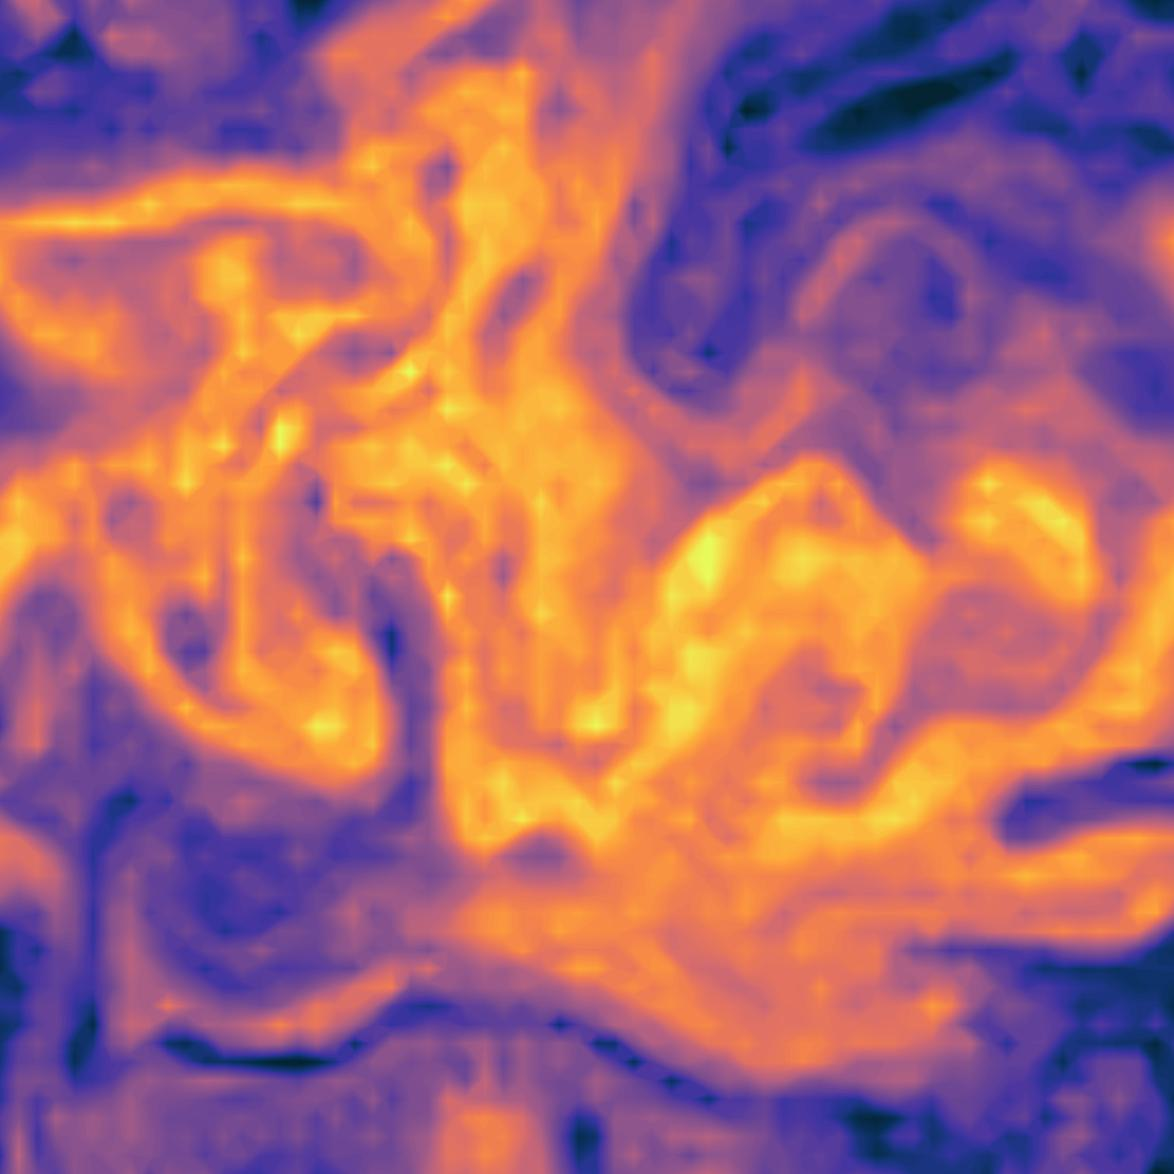
\includegraphics[width=.74\textwidth]{../../figures/theta-z0.jpg}
        };
        \draw [line width=5pt,
            {Stealth}-{Stealth}]
            ($ (lower.south west) + (0.45, 0.0) $)
            --
            ($ (lower.south east) - (0.45, 0.0) $)
            node [midway, yshift=-0.75em] {$N_x = 64$};
        \draw [line width=5pt,
            {Stealth}-{Stealth}]
            ($ (upper.south west) + (0.0, 0.45) $)
            --
            ($ (upper.north west) - (0.0, 0.45) $)
            node [midway, xshift=-0.75em, rotate=90] {$N_y = 64$};
        \draw [line width=5pt,
            {Stealth}-{Stealth}]
            (upper.south west)
            --
            (lower.south west)
            node [midway, xshift=-0.5em, yshift=-0.5em, rotate=-45] {$N_z = 2$};
    \end{tikzpicture}
\end{minipage}
\begin{minipage}{.39\textwidth}
    \begin{itemize}
        \item Blumen model of Eady turbulence, as presented in\\
            \cite{tulloch_note_2009}
        \item 15 years: training and validation
        \item 5 years: testing
        \item 5 years: separation
    \end{itemize}
\end{minipage}

    \end{FlushLeft}
}{

    \begin{FlushLeft}
        \section{Nonlinear Vector Auto-Regression}

\vspace{1em}
\begin{minipage}{\textwidth}
    \centering
    \begin{tikzpicture}[scale=1]

        % --- State vectors
        \node(tm1) at (-12, 6){
            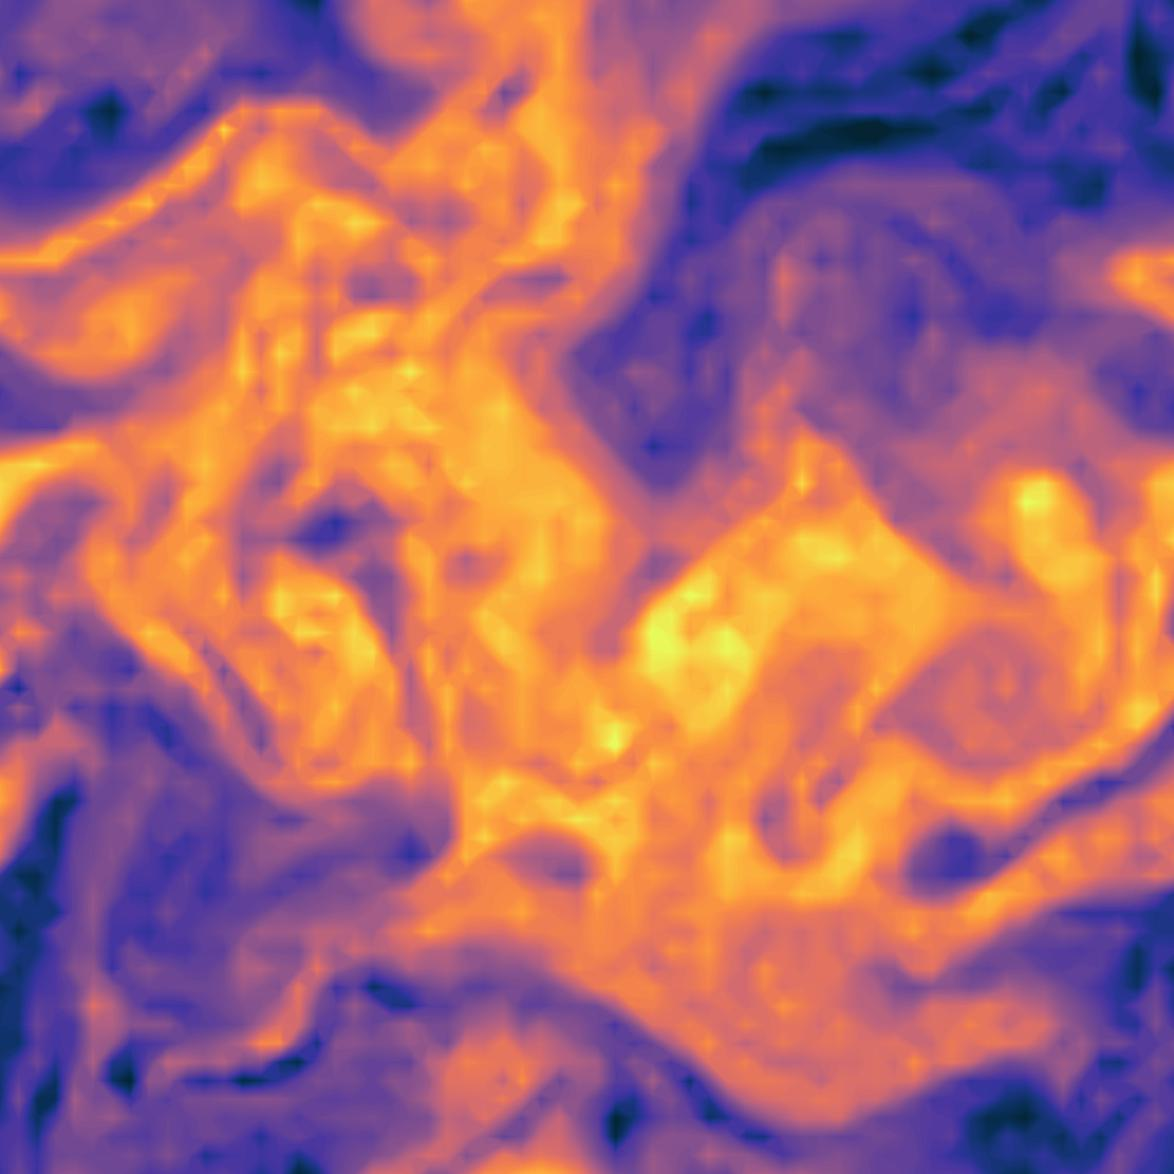
\includegraphics[width=.22\textwidth]{../../figures/theta-t-1.jpg}
        };
        \node at
            ($ (tm1.north) + (0.0, 0.5) $)
            {$\inputstate(t-N_\text{lag})$};

        \node at (-6, 6) {$\bullet\,\,\bullet\,\,\bullet$};

        \node(t0) at (0, 6){
            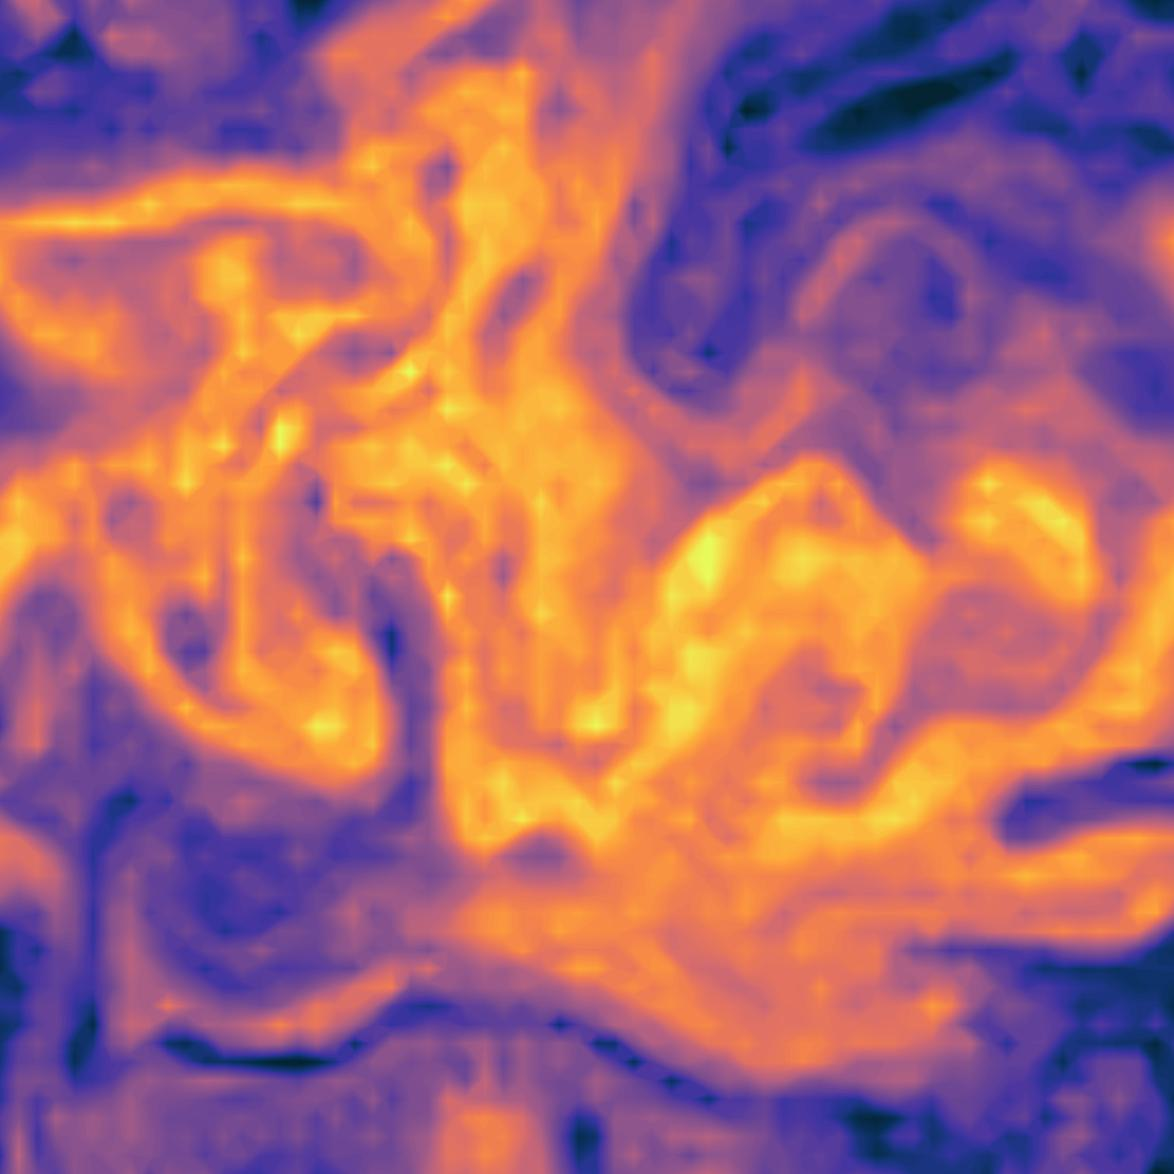
\includegraphics[width=.22\textwidth]{../../figures/theta-z0.jpg}
        };
        \node at
            ($ (t0.north) + (0.0, 0.5) $)
            {$\inputstate(t)$};

        \node(tp1) at (8, 6){
            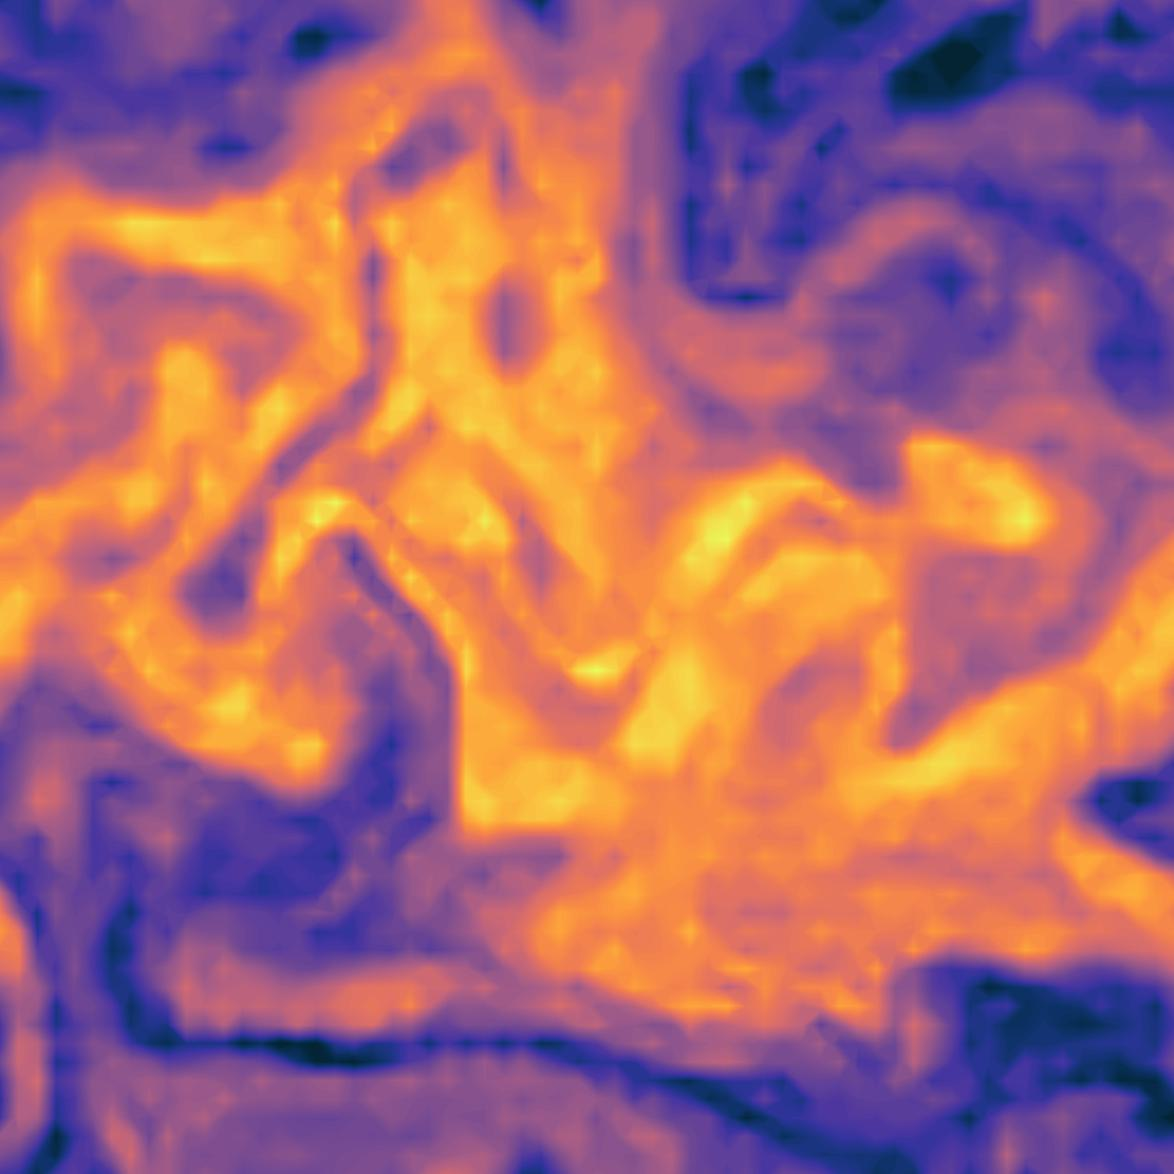
\includegraphics[width=.22\textwidth]{../../figures/theta-t1.jpg}
        };
        \node at
            ($ (tp1.north) + (0.0, 0.5) $)
            {$\inputstate(t+1)$};

        % --- RNN
        \node[rectangle,
            draw=black,
            minimum height=7.5em,
            minimum width=2em,
            line width=3pt,
            draw opacity=1,
            rounded corners=.5em] (rnn) at (8, -6) {};
        \node[circle,
            fill=sapphire,
            minimum height=0.5em,
            fill opacity=1] at (8, -3) {};
        \node[circle,
            fill=sapphire,
            minimum height=0.5em,
            fill opacity=1] at (8, -5) {};
        \node[circle,
            fill=sapphire,
            minimum height=0.5em,
            fill opacity=1] at (8, -7) {};
        \node[circle,
            fill=sapphire,
            minimum height=0.5em,
            fill opacity=1] at (8, -9) {};
        \node at
            ($ (rnn.south) - (0.0, 1.0) $) {$\hidden(t+1)$};

        % --- Connections
        \draw[line width=8pt, -{Stealth}, draw=gray]
            (t0.south) to [out=-90, in=-180] (rnn.west);
        \draw[line width=8pt, -{Stealth}, draw=gray]
            (tm1.south) to [out=-90, in=-180] (rnn.west);
        \draw[line width=8pt, -{Stealth}, draw=emerald]
            (rnn.north) to (tp1.south);

    \end{tikzpicture}
\end{minipage}


\begin{itemize}
    \item Build next hidden state, $\hidden(t+1)$, explicitly from input state
        at current and previous timesteps:
        $\{\inputstate(t), ..., \inputstate(t-N_\text{lag})\}$
    \item Here, consider quadratic relation between\\neighboring grid cells
    \item Map hidden state to target state
        \begin{equation*}
            \inputstate(t+1) = \Wout \hidden(t+1)
        \end{equation*}
        via trained readout matrix:
        \vspace{.5em}
        \begin{equation*}
            \Wout \coloneqq \argmin \left\{
                \dfrac{1}{2}\sum_{n=1}^{\ntrain} \norm{\Wout \hidden_n - \state_n}^2
                +
                \dfrac{\tikhonov}{2}\norm{\Wout}_\text{F}^2 \, \right\}
        \end{equation*}
    \item Note: hidden space is larger than input/target space
\end{itemize}

\vspace{1em}
\begin{minipage}{\textwidth}
    \centering
    \begin{tikzpicture}[scale=1]

        % --- State vectors
        \node(tm1) at (-8, 0){
            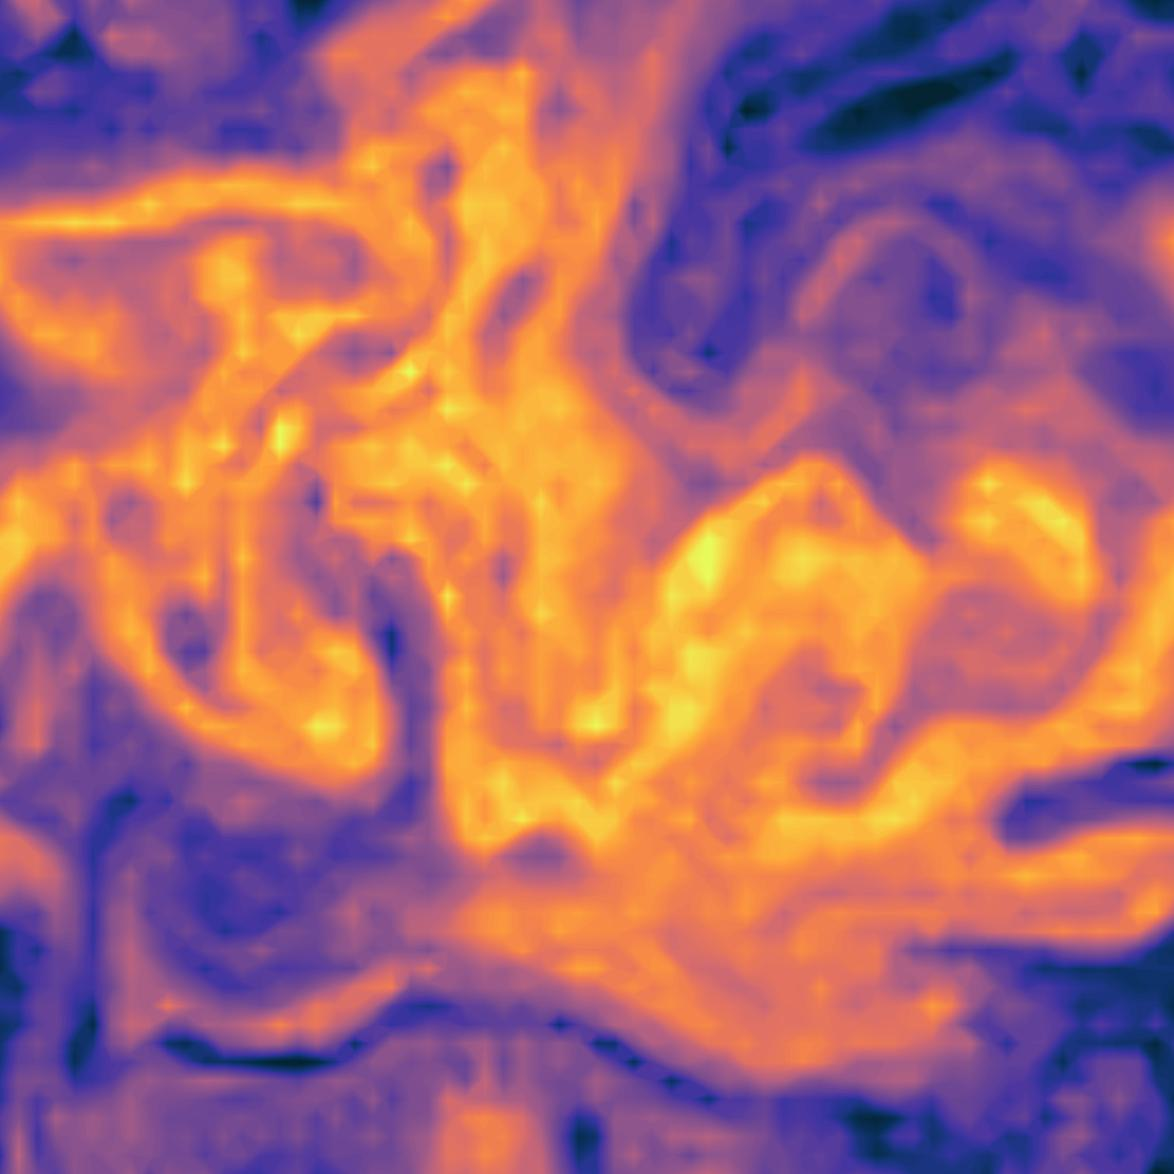
\includegraphics[width=.22\textwidth]{../../figures/theta-z0.jpg}
        };
        \node(tp1) at (8, 0){
            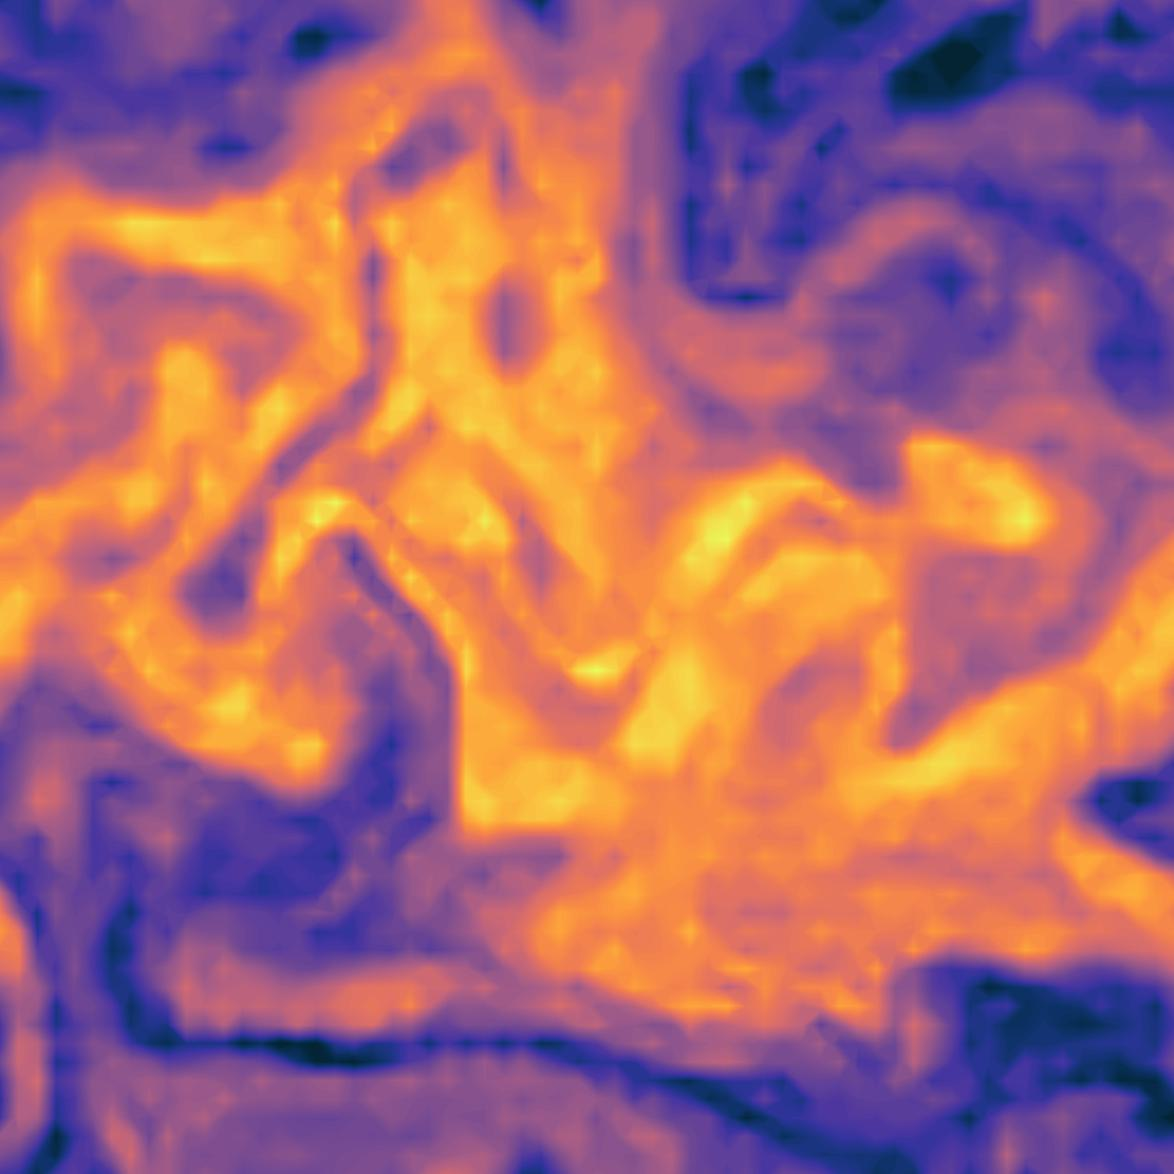
\includegraphics[width=.22\textwidth]{../../figures/theta-t1.jpg}
        };

        % --- RNN
        \node[rectangle,
            draw=black,
            minimum height=7.5em,
            minimum width=2em,
            line width=3pt,
            draw opacity=1,
            rounded corners=.5em] (rnn) at (0, 0) {};
        \node[circle,
            fill=sapphire,
            minimum height=0.5em,
            fill opacity=1] at (0, 3) {};
        \node[circle,
            fill=sapphire,
            minimum height=0.5em,
            fill opacity=1] at (0, 1) {};
        \node[circle,
            fill=sapphire,
            minimum height=0.5em,
            fill opacity=1] at (0, -1) {};
        \node[circle,
            fill=sapphire,
            minimum height=0.5em,
            fill opacity=1] at (0, -3) {};

        % --- Mappings
        \node[trapezium,
            fill=gray,
            fill opacity=1,
            minimum width=7.25em,
            minimum height=2em,
            trapezium angle=80,
            trapezium stretches=true,
            rotate=90] at (-3, 0) {};

        \node[trapezium,
            fill=emerald,
            fill opacity=1,
            minimum width=7.25em,
            minimum height=2em,
            trapezium angle=80,
            trapezium stretches=true,
            rotate=-90] at (3, 0) {};
    \end{tikzpicture}
\end{minipage}

\vspace{1em}
\hfill\begin{minipage}{0.97\textwidth}
    so we implement a parallization strategy akin to standard domain
    decomposition in GCMs
\end{minipage}

\section{References}
\vspace{1em}
\begin{minipage}{\textwidth}
    \fontsizeinstitution
        \citeps{pathak_using_2017} doi: 10.1063/1.5010300 \\
        \citeps{platt_systematic_2022} doi: 10.1016/j.neunet.2022.06.025 \\
        \citeps{penny_integrating_2022} doi: 10.1029/2021MS002843 \\
        \citeps{tulloch_note_2009} doi: 10.1175/2008JAS2921.1 \\
        \citeps{zhang_catch-22_2022} doi: 10.48550/ARXIV.2210.10211
\end{minipage}

    \end{FlushLeft}
    %\nobibliography{../references.bib}
    \bibstyle{apa}
    %\bibliographystyle{apa}
}
\end{document}
